\chapter{Introduction}
\label{chapter1}

%%%%%%%%%%%%%%%%%%%%%%%%%%%%%%%%%%%%%%%%%%%%%%%%%%%%%%%%%%%%%%%%%%%%%%%

The main objective of a network is to provide communications between two or more desired endpoints. But over time, as networks have become larger and more complex so did their functions grown as well, in such a manner, that nowadays they may also include traffic integrity and survivability aspects and also network management and performance monitoring \cite{Telecommunications}. Until recently in the history of mankind, communications were very limited, for instance by geographical proximity as messages were transported by messengers or couriers, who either walked or were transported by domesticated animals, or were sent through fire, smoke or sound signals, but in this particular cases just confirming prearranged messages. In the new telecommunications era this master-to-servant relationship was eradicated, replacing the service of a messenger by mechanical telegraphs, followed by copper wires and electromagnetic waves and most lately by the revolutionary optical fibers. These advances dramatically reduced the time required to transport messages, accelerated business transactions, and so in a manner improved human relationships by allowing real-time worldwide communications \cite{Telecommunications}. \par Networks are in its essence, very complex engineering systems with many variables to take into account. More precisely, an optical network is a type of data communication network built with optical fiber technology and is composed of fiber optic cables that carry channels of light, combined with equipment deployed along the fibers to process it. Major breakthrough technologies development has been followed by the evolution of optical networks. For instance, one of the earliest technological advances was the ability to carry multiple channels of light on a single fiber optic cable, where each light stream is carried at a different optical frequency and multiplexed into a single fiber, the so called \gls{wdm} \cite{SimmonsJane2008}. Until recently, telecommunication networks have been an intelligent combination of transmission and switching technologies, and even if transmission and switching are still the basic building blocks of any network, their fundamentals nowadays cover a much complex and broader scope mainly due to the arise of digital technologies which introduced packet switched networks, which proved to have superior performance regarding various aspects such as connection time, reliability, economy, flexibility and much more \cite{doi:10.1002/9780470683576.ch1}. In this last, there is a dynamic allocation of the transmission bandwidth, allowing many users to share the same transmission line and thus reducing the wastage of available bandwidth resources, in contrast to old circuit switched networks where the same was pre-allocated. %Currently, the leading communication protocol used to transmit signals over optical fiber links is defined by ITU-T, as \gls{otn} and integrates transport for all digital payloads with superior performance relatively to previous optical \gls{wdm} transport solutions, namely \gls{sonet} and \gls{sdh}.

 
\par A common way to geographically divide telecommunication networks is in access, metro and core networks, being the last two almost entirely based on optical fiber technology, although the penetration of optical fiber communications in the access segment is progressing at an astonishing rate \cite{F-T-H}. Access networks usually connect directly to end users, providing interfaces that operate at bit-rates suitable to support various different applications and typically cover a small geographical area, spanning the last tens of kilometers to the end user \cite{7127266}. On the other hand, metro networks aggregate traffic from several access networks and carry it between major cities, countries or continents. Finally, core networks who are also named transport or backbone networks cover an even larger geographical area, typically thousands of kilometer, and may be shared among millions of customers \cite{SimmonsJane2008}\cite{anpinto}. 
\par Devices and connection demands to the Internet have been growing unbelievably fast mainly due to the expansion of optical fiber to customers homes, the increased bandwidth of new mobile technologies, video traffic, and business virtual private networks with remote access to huge databases, which also translates in a growth in Internet-based applications \cite{SimmonsJane2008}\cite{TiagoEsteves}. Each year, various new devices in different form factors with increased capabilities and intelligence are introduced and adopted in the market. All of this results in a major increase  of \gls{ip} traffic as we can see in figure \ref{cisco11}. In response, as operators are undergoing a heavy pressure to reduce the cost per bit transported, they have been investing in a widespread of upgrades  to their metro and backbone networks, introducing new technologies, to greatly enhance their capacity and reduce expenses. Currently carriers are demanding \gls{wdm} optical networking technologies that provide both low \gls{capex} and low \gls{opex} and as almost all traffic is transported through optical networks the operators are very interested in reducing the cost per transported bit as much as possible without compromising the \gls{qos} \cite{SimmonsJane2008}.
\vspace{11pt}

\begin{figure}[H]
  \begin{center}
    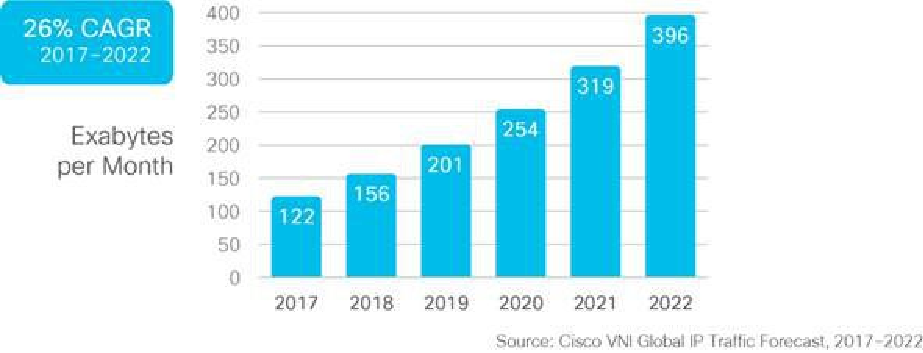
\includegraphics[width=0.6\textwidth]{fig/logos/ciscoForecast.pdf}
    \caption{Cisco forecasts per month of IP traffic from 2017 until 2022 \cite{ciscoForecast}.}
     \label{cisco11}
  \end{center}
\end{figure}


\newpage
%%%%%%%%%%%%%%%%%%%%%%%%%%%%%%%%%%%%%%%%%%%%%%%%%%%%%%%%%%%%%%%%%%%%%%%%
\section{Motivation}
\label{motivation}

The widespread of telecommunications worldwide is the result of the ability to place in the market services at lower prices easily affordable by the masses. The cost factor is therefore, a major enabling issue in the telecommunications industry and tend to have a strong influence in all engineering and administrative decisions, once it directly affects the competitiveness of system vendors and network operators \cite{anpinto}. Network planning tasks such as, how to route and protect traffic in a network or how to bundle different traffic into the same wavelengths, must usually be performed or at least assisted by software tools, the so-called network planning tools. This happens because of the extreme difficulty to make a fast and scalable manual planning to a large and complex telecommunication network \cite{SimmonsJane2008}. Thus, network planning tools are extremely important as they are used in the various stages of the telecommunications business, namely, in the budgeting, implementation and operation stages enabling the optimization of the available resources and significant cost savings \cite{RuiMoraisPhD}. Currently, there exists various commercial network planning tools but as they usually take into account specialized implementation constraints or proprietary technology to those companies, they are usually not available for public research and comparative studies \cite{7193723}. In this context, the development of methodologies and optimization tools for transport networks planning is being intensively investigated in academia environments. Therefore, arose the interest and opportunity to develop a global platform that serves as a planning tool created along this dissertation, which is meant for academic and educational research purposes. Additionally, some heuristic algorithms were developed from scratch, implemented and validated in that same platform, offering near optimal solutions in shortest periods of time (for highly complex problems) when compared with other methods, for instance the \gls{ilp} models. These algorithms often need to balance solution quality and scalability, as this last criterion poses a problem for ILP based algorithms, which are known to scale poorly with the problem size, the less complex heuristic algorithms can be considered as a great advantage.

%%%%%%%%%%%%%%%%%%%%%%%%%%%%%%%%%%%%%%%%%%%%%%%%%%%%%%%%%%%%%%%%%%%%%%%%
\section{Objectives}
\label{objectives}
Due to the importance of transport network planning and dimensioning, this dissertation aims to achieve the following main objectives:

\begin{enumerate}
  \item Elaborate a generic framework for optical transport networks dimensioning based on heuristics.
  \item Implement the framework recurring to the NetXPTO-NetPlanner simulator.
  \item Develop heuristic algorithms for transparent networks.
  \item Elaborate an economic comparative study and validate the heuristics with ILP and analytical results.
\end{enumerate}


%%%%%%%%%%%%%%%%%%%%%%%%%%%%%%%%%%%%%%%%%%%%%%%%%%%%%%%%%%%%%%%%%%%%%%%%%%%%%%%%%%%%%%%
\section{Dissertation outline}
\label{outline}

This dissertation is organized in 7 chapters. Chapter \ref{chapter2} serves the purpose of a state-of-the-art review on optical transport networks dimensioning. The chapter introduces and explains the main concepts and notions used throughout the dissertation, it starts by giving a general description of the architecture and possible topologies of optical networks as well as a description of the reference and realistic networks and the different traffic scenarios defined. The remaining of the chapter is devoted to the detailed description of the models used for \gls{capex} estimations, namely the analytical, the ILP and the Heuristic. Chapter \ref{chapter3} is composed of several sections, where a general description of the created generic framework is presented as well as of each of the individual entities that it is comprised of. Afterwards, in chapter \ref{chapter4}, is taken an approach on the practical implementation of the created platform through NetXPTO-Netplanner simulator, the set of variables and inputs used is extensively detailed as well as the functionalities and features provided. In chapter \ref{chapter5} the implemented heuristic algorithms are explored and other possible alternatives to the strategies adopted are provided. Some charts representing the pseudo code behind the routing, grooming and wavelength assignment are also present in this chapter. Chapter \ref{chapter6} contains the results obtained throughout this dissertation for both the reference and the realistic networks. Also in this chapter a comparative analysis is performed with the results obtained wit different methods.  Finally, in chapter \ref{chapter7} some conclusions and suggestions for future research directions are provided.

%%%%%%%%%%%%%%%%%%%%%%%%%%%%%%%%%%%%%%%%%%%%%%%%%%%%%%%%%%%%%%%%%%%%%%%%%%%%%%%%%%%%%%%%%%%%%%%%%%%%%%%%%%%%%%%%%%%%%%%%%%%%%

\section{Major Achievements}

The list of main objectives and contributions achieved during this dissertation are presented below:

\begin{enumerate}
\item Creation of a generic framework for optical networks dimensioning.
\item Implementation of the framework over the NetXPTO-Netplanner simulator, resulting in an operational platform.
\item Successful testing and validation of the developed heuristic algorithms.
\end{enumerate}

